\documentclass[12pt]{article}

\usepackage{fullpage}
\usepackage{mdframed}
\usepackage{colonequals}
\usepackage{algpseudocode}
\usepackage{algorithm}
\usepackage[most, breakable]{tcolorbox}
\usepackage[all]{xy}
\usepackage{proof}
\usepackage{mathtools}
\usepackage{bbm}
\usepackage{amssymb}
\usepackage{amsthm}
\usepackage{amsmath}
\usepackage{amsxtra}
\usepackage{enumitem}
\newcommand{\bb}{\mathbb}


\newtheorem{theorem}{Theorem}[section]
\newtheorem{theorem*}{Theorem}
\newtheorem{definition}[theorem]{Definition}
\newtheorem{corollary}{Corollary}[theorem]
\newtheorem{lemma}[theorem]{Lemma}
\newtheorem{prop}[theorem]{Proposition}
\newtheorem{remark}[theorem]{Remark}


\newtheorem*{exercisehelper}{Exercise.}
\newenvironment{exercise}[1]{%
  \IfBlankTF{#1}
    {\renewcommand{\exercisehelper}{\textbf{Exercise} \unskip}}
    {\renewcommand\exercisehelper{\textbf{Exercise #1}}}%
  \exercisehelper
}{\endexercisehelper}

\theoremstyle{remark}
\newtheorem*{solution}{Solution}
\newcommand{\mathcat}[1]{\textup{\textbf{\textsf{#1}}}} % for defined terms

\newenvironment{problem}[1]
{ \begin{tcolorbox}[breakable]\noindent\textbf{Problem #1}.}
{\vskip 6pt \end{tcolorbox}}

\newenvironment{enumalph}
{\begin{enumerate}\renewcommand{\labelenumi}{\textnormal{(\alph{enumi})}}}
{\end{enumerate}}

\newenvironment{enumroman}
{\begin{enumerate}\renewcommand{\labelenumi}{\textnormal{(\roman{enumi})}}}
{\end{enumerate}}

\newcommand{\defi}[1]{\textsf{#1}} % for defined terms



\setlength{\hfuzz}{4pt}

\let\H\relax
\let\P\relax
\newcommand{\H}{\mathbb H}
\newcommand{\P}{\mathbb P}
\newcommand{\C}{\mathbb C}
\newcommand{\N}{\mathbb N}
\newcommand{\Q}{\mathbb Q}
\newcommand{\R}{\mathbb R}
\newcommand{\Z}{\mathbb Z}
\newcommand{\F}{\mathbb F}
\newcommand{\br}{\mathbf{r}}
\newcommand{\RP}{\mathbb{RP}}
\newcommand{\CP}{\mathbb{CP}}
\newcommand{\nbit}[1]{\{0, 1\}^{#1}}
\newcommand{\bits}{\{0, 1\}^{n}}
\newcommand{\bbni}{\bigbreak \noindent}
\newcommand{\norm}[1]{\left\vert\left\vert#1\right\vert\right\vert}
\newcommand{\dbar}{\overline{\partial}}
\let\d\relax
\newcommand{\d}{\partial}
\newcommand{\calO}{\mathcal{O}}
\newcommand{\calF}{\mathcal{F}}
\newcommand{\calG}{\mathcal{G}}
\newcommand{\calH}{\mathcal{H}}
\newcommand{\calE}{\mathcal{E}}
\newcommand{\calC}{\mathcal{C}}
\newcommand{\calD}{\mathcal{D}}

\let\1\relax
\newcommand{\1}{\mathbf{1}}
\newcommand{\fr}[2]{\left(\frac{#1}{#2}\right)}
\newcommand{\todo}[1]{\textcolor{red}{\textbf{TODO:} #1}}
\newcommand{\vecz}{\mathbf{z}}
\newcommand{\vecr}{\mathbf{r}}
\DeclareMathOperator{\Cinf}{C^{\infty}}
\DeclareMathOperator{\Id}{Id}
\DeclareMathOperator{\Ell}{Ell}
\DeclareMathOperator{\CL}{\mathcal{CL}}

\DeclareMathOperator{\Alt}{Alt}
\DeclareMathOperator{\Aut}{Aut}
\DeclareMathOperator{\ann}{ann}
\DeclareMathOperator{\codim}{codim}
\DeclareMathOperator{\End}{End}
\DeclareMathOperator{\Hom}{Hom}
\DeclareMathOperator{\id}{id}
\DeclareMathOperator{\M}{M}
\DeclareMathOperator{\Mat}{Mat}
\DeclareMathOperator{\Ob}{Ob}
\DeclareMathOperator{\opchar}{char}
\DeclareMathOperator{\opspan}{span}
\DeclareMathOperator{\rk}{rk}
\DeclareMathOperator{\sgn}{sgn}
\DeclareMathOperator{\Sym}{Sym}
\DeclareMathOperator{\tr}{tr}
\DeclareMathOperator{\img}{img}
\DeclareMathOperator{\coker}{coker}
\DeclareMathOperator{\Spec}{Spec}
\DeclareMathOperator{\CandE}{CandE}
\DeclareMathOperator{\CandO}{CandO}
\DeclareMathOperator{\argmax}{argmax}
\DeclareMathOperator{\first}{first}
\DeclareMathOperator{\last}{last}
\DeclareMathOperator{\cost}{cost}
\DeclareMathOperator{\dist}{dist}
\DeclareMathOperator{\path}{path}
\DeclareMathOperator{\parent}{parent}
\DeclareMathOperator{\argmin}{argmin}
\DeclareMathOperator{\excess}{excess}
\let\Pr\relax
\DeclareMathOperator{\Pr}{\mathbf{Pr}}
\DeclareMathOperator{\Exp}{\mathbb{E}}
\DeclareMathOperator{\Var}{\mathbf{Var}}
\let\limsup\relax
\DeclareMathOperator{\limsup}{limsup}
%Paired Delims
\DeclarePairedDelimiter\ceil{\lceil}{\rceil}
\let\oldceil\ceil
\renewcommand{\ceil}[1]{\oldceil*{#1}}

\DeclarePairedDelimiter{\floor}{\lfloor}{\rfloor}
\let\oldfloor\floor
\renewcommand{\floor}[1]{\oldfloor*{#1}}





\newcommand{\dagstar}{*}

\newcommand{\tbigwedge}{{\textstyle{\bigwedge}}}
\setlength{\parindent}{0pt}
\setlength{\parskip}{5pt}


\usepackage{listings}
\usepackage{courier}
\usepackage{microtype}


\lstset{
  basicstyle=\footnotesize\ttfamily,
  breaklines=true,
  breakatwhitespace=true
  columns=fullflexible,
  keepspaces=true,
  frame=single,
  escapeinside={(*@}{@*)}
}
\usepackage{tikz}
\usetikzlibrary{calc} 

\begin{document}

\title{Math 71: Abstract Algebra}

\author{Prishita Dharampal}
\date{}
\maketitle

\begin{problem}{1}
Archimedes discovered a construction that trisects any given angle using a compass and a “marked” straightedge. This straightedge has two special markings a distance $1$ apart.
The straightedge can be placed so that it passes through any already drawn point and such that both markings intersect other already drawn lines or circles.
\begin{center}
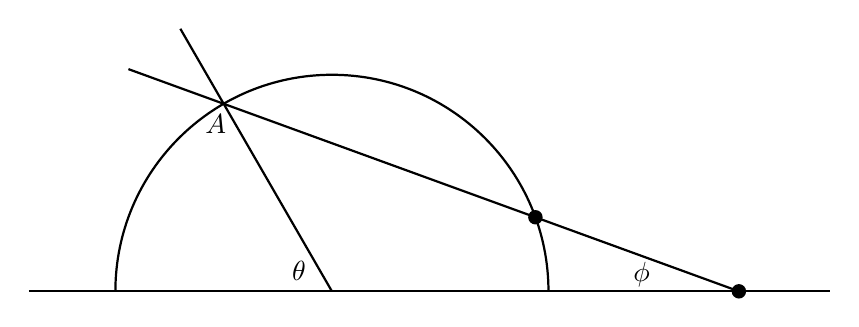
\begin{tikzpicture}[scale=2.75,thick]
\draw (-1.4cm,0) -- (2.3cm,0);
\draw (1cm,0) arc (0:180:1cm);
\draw (0,0) -- (120:1.4);
\draw (${2*cos(20)}*(1,0)$) -- +(160:3cm);
\draw (0,0) node[anchor=south east,xshift=-2mm,yshift=0mm] {$\theta$};
\draw (${2*cos(20)}*(1,0)$) node[anchor=south east,xshift=-10mm,yshift=-.8mm] {$\phi$};
\draw (120:1) node[anchor=north,xshift=-1mm,yshift=0mm] {$A$};
\draw[fill=black] (${2*cos(20)}*(1,0)$) circle (0.8pt);
\draw[fill=black] (20:1cm) circle (0.8pt);
\end{tikzpicture}
\end{center}

In the picture, start with a horizontal line and another line meeting it with angle $\theta$. Draw a circle of radius $1$ around the intersection point of these two lines. The other line meets the circle at point $A$. Then place the marked straightedge so that it passes through the point $A$ and such that the markings intersect the circle and the horizontal line. Prove that the angle $\varphi$ that the straightedge makes with the horizontal line is equal to $\theta/3$.
\end{problem}

\begin{problem}{2}
Prove that any angle $\theta$ such that $\tan(\theta)$ is rational can be constructed with compass and straightedge. Prove that such angles are dense in the interval $(-\pi/2,\pi/2)$.
\end{problem}

\begin{problem}{3}
Prove that an angle $\theta$ can be trisected using compass and straightedge if and only if the polynomial
\[
4x^3 - 3x - \cos(\theta)
\]
is reducible over $\mathbb{Q}(\cos(\theta))$.

\textbf{Bonus.} Choose your favorite trisectable angle $\theta$, and describe a step-by-step construction that performs the trisection; saying “I start with $\theta/3$ then triple it to make $\theta$ then I already have $\theta/3$ so I'm done” is cheating.
\end{problem}

\begin{problem}{4}
To $5$-sect an angle means to divide it by $5$.
\begin{enumerate}
\item Prove that the angles $2\pi$, $\pi$, $2\pi/3$, and $\pi/2$ can be $5$-sected by compass and straightedge.
\item Prove that a general angle cannot be $5$-sected by compass and straightedge.
\end{enumerate}
\end{problem}

\begin{problem}{5}
Let $p$ be an odd prime.
\begin{enumerate}
\item Prove that both $\mathbb{Q}(\zeta_p)$ and $\mathbb{Q}(\zeta_{2p})$ have degree $p-1$ over $\mathbb{Q}$.
\item Prove that both $\mathbb{Q}(\cos(2\pi/p))$ and $\mathbb{Q}(\cos(\pi/p))$ have degree $(p-1)/2$ over $\mathbb{Q}$.
\item Find the minimal polynomial of $\cos(2\pi/9)$ over $\mathbb{Q}$ and prove that it splits completely over $\mathbb{Q}(\cos(2\pi/9))$.
\end{enumerate}
\end{problem}

\begin{problem}{6}
For $3 \le n < 17$, determine whether a regular $n$-gon can be constructed by compass and straightedge. 
\end{problem}

\end{document}